\documentclass[a4paper,12pt]{article}

% Se vuoi che il pdf sia in formato mobile, decommenta la linea qui sotto e commenta la prima linea del codice
%\input{../../.Latex_stuff/mobile.tex}

\input{../../.Latex_stuff/commands.tex}



\sloppy
\begin{document}

\begin{titlepage}
\begin{center}
	\Large{\textbf{Appunti di Sviluppo Software in Gruppi di Lavoro Complessi}}
\vfill
\normalsize{Caccaro Sebastiano}\\
\normalsize{A.A.2019/2020}
\end{center}
\end{titlepage}
\tableofcontents

\clearpage


%Lezione di Giovedi 4 Ottobre 2019
\lessonDate{4 Ottobre 2019}
\section{Modelli Organizzativi}
Lo sviluppo software presenta dei problemi intrinseci:
\begin{itemize}
\item \textbf{Non linearità del software}: Un errore molto piccolo può avere conseguenze catastrofiche
\item Obiettivi poco chiari e mutabili
\end{itemize}
Questi problemi esistono tutt'oggi e sono difficilmente mitigabili. Esistono invece delle criticità che possono essere risolte.

\definition{Legge di Brooks}{Aggiungere personale ad un progetto in ritardo lo farà solo ritardare.}

Nello sviluppo software, non tutto è facilmente parallelizzabile. Non posso far nascere un bambino da 9 donne in un mese. Va da se che l'\textbf{effort} non corrisponde al \textbf{progress}. \`E molto facile stimare quanto si è lavorato, è meno facile misurare di quanto si è progredito, e questo può causare ulteriori ritardi. La soluzione non è aggiungere personale.

Un progetto deve mantenere sempre la sua \textbf{integrità concettuale}.\\
Per far ciò Brooks propone vari modelli.

\subsection{Modelli a Cattedrale e sala Operatoria}
\begin{itemize}
\item \textbf{Cattedrale}: Tenere rigorosamente separata progettazione e implementazione. L'implementatore deve quindi curarsi solamente di seguire quanto progettato. Si mantiene così la visione originale del progetto. Questo modello ha però il difetto di essere molto poco flessibile, e difetti nel progetto comportano problematiche enormi.
\item \textbf{Sala operatoria:} Solamente il chirurgo (superbravo) si occupa di fare le cose importanti, gli altri nella sala fanno praticamente solo da assistente. Il vero lavoro viene svolto solamente dal chirurgo (una sola persona).
\end{itemize}
Questi modelli fanno però due grosse supposizioni:
\begin{itemize}
\item Che sia possibile accentare lo sforzo creativo in un'unica persona.
\item Che sia possibile separare completamente progettazione e implementazione.
\end{itemize}
La maggior parte delle volte, tuttavia, queste supposizioni non si rivelano corrette.

\subsubsection{Critiche}
Eric Raymond contrappone il modello a \textbf{bazaar} (usato per lo sviluppo di Linux) contro la cattedrale di Brooks, osservando che il modello open source di Linux produca software di qualità, pur non usando i modelli proposti da brooks.
\lessonDate{8 Ottobre 2019}

\subsection{Modello a Bazaar}
Usato in Linux, si identifica esplicitamente come l'antitesi del modello a cattedrale. Raymond condivide l'analisi di Brooks, ma arriva alla conclusione che ci possano essere altri modelli in certe situazioni.
\definition{Baazar}{Mercato autogestito, dove chiunque può mettere una bancarella dove vuole, quando vuole}

\begin{figure}[H]
	\centering
	 \includegraphics[width=0.6\linewidth]{Immagini/bazaar.jpg}
	 \caption{Un bazaar}
\end{figure}

Nel modello a Baazar, ognuno fa i propri interessi e sviluppa ciò che gli interessa sviluppare. Non c'è quindi un obiettivo comune, ma nel perseguire i propri interessi chi sviluppa nel modello a Baazar contribuisce a tenere viva la codebase. Questo processo non segue un modello prefissato, e quindi produce una sorta di organismo in continua evoluzione, il quale scopo quindi non diventa obsoleto.
Ma cosa permette a progetti come questi, che non adottano i modelli di Brooks, di non fallire?
\begin{itemize}
 \item Le persone non lavorano perchè costrette a farlo per un'azienda. Chi contribuisce lo fa per interessi personali, ed è quindi interessato e motivato ("personal itch")
 \item Gli utenti sono considerati co-sviluppatori, ciò aiuta a individuare e risolvere bug più velocemente
 \item Rilasciare presto e frequentemente, in modo tale da avere sempre feedback
\end{itemize}

\definition{Legge di Linux}{Data una base di beta-tester e co-sviluppatori abbastanza amplia, quasi ogni problema può essere scoperto e risolto velocemente da qualcuno.}

Per Brooks un numero elevato di utenti porta inevitabilmente ad avere più bug, in quanto ogni utente può vedere problemi diversi. Raymond invece considera gli utenti come collaboratori, che possono aiutare lo sviluppatore.\\
Anche questo modello, in teoria fantastico, in pratica è abbastanza idealistico.

\subsection{Modello a Kibbutz}
Per poter supportare delle applicazioni, un sistema deve fornire dei servizi adeguati, come kernel, driver, librerie di sistema ecc.\\
Linux è solamente un kernel, non ci si possono far girare applicazioni. Nasce quindi li concetto di \textbf{distribuzione}, ovvero un sistema completo immediatamente utilizzabile. Un programma viene quindi distribuito sotto forma di pacchetto, che è progettato per lavorare con una distribuzione (esempio pacchetto .deb).

\definition{Kibbutz}{Fattoria, villaggio, impresa collettiva nata in Israele, con scopo di popolare il nuovo stato}

\begin{figure}[H]
	\centering
	 \includegraphics[width=0.6\linewidth]{Immagini/kibbutz.jpg}
	 \caption{Un kibbutz}
\end{figure}

Non parliamo quindi più di un bazaar, dove ognuno fa quello che vuole. Ma di un'organizzazione strutturata e organizzata, con uno scopo comune. Sono presenti delle \textbf{policy} prestabilite, che hanno dei corrispettivi tool che assicurano il rispetto di tali policy. Queste policy hanno l'effetto di abbassare drasticamente l'effort comunicativo fra i vari contributori al progetto. Praticamente molti progetti open-source sono organizzati a kibbutz, perchè il modello a Baazar non è una strada viabile. 
\\Questa è la filosofia adottata da Debian.

\subsubsection{Esempio di Debian}
Fin dall'inizio, Debian è openSource (ad oggi circa 1900 sviluppatori, che devono superare degli esami). Supporta più di 10 architetture e tre kernel diversi (una distribuzione non è per forza linux).\\
In Debian, ogni pacchetto contiene alcune informazioni come:
\begin{itemize}
 \item Nome
 \item Architetture supportate
 \item \textbf{Dipedenze}: tutti i pacchetti che servono al corretto funzionamento del mio pacchetto. Il solo codice sorgente del mio pacchetto è inutile senza queste informazioni
\end{itemize}

Nel pacchetto sono contenuti anche i propri file di configurazione. Questi file sono specificati nei pacchetti, quindi un upgrade non va a intaccare la configurazione. In caso ci siano problemi, chiedo all'utente di fare il merge.

\lessonDate{10 Ottobre}
\section{Metodologie Agili}
Negli anni 90 si pensa che il modo per aumentare la qualità di processi debba dipendere da una gran enfasi sulla produzione di documentazione, UML ecc. Secondo gli agilisti, tutto il focus che viene posto sui processi non risulta effettivamente in software di qualità.\\ Nascono quindi dei nuovi modelli organizzativi che reagiscono a queste cose pallose, come:
\begin{itemize}
\item eXtreme Programming
\item Scrum
\end{itemize}
Il manifesto della \textbf{Programmazione Agile} viene pubblicato nel 2001, ed esprime i seguenti concetti:
\begin{enumerate}
\item Individui e interazioni \textgreater\space Processi e strumenti
\item Software funzionante \textgreater\space Documentazione esaustiva
\item Collaborazione cliente \textgreater\space Negoziazione contratti
\item Rispondere al cambiamento \textgreater\space Seguire un piano
\end{enumerate}
Tutti questi punti sono un però \textbf{molto generici e idealistici}, e sono sì belli, ma poco applicabili. Il più concreto di questi è forse il punto 4, perchè riconosce il fatto che è molto facile sbagliare la pianificazione. \E meglio quindi salvare risorse per potersi adattare a nuove situazioni.
\lessonDate{15 Ottobre 2019}
\vspace{0.5cm}
\noindent Al contrario di quanto si è portati a pensare, agile non significa il rifiuto dei processi, ma piuttosto il rifiuto di continue verifiche e benchmark come misura della qualità di quanto prodotto. Quello che fanno gli agilisti è sostituire al canone fatto di processi e misurazioni un canone con dei principi astratti più o meno condivisibili.

\subsection{Principi agile}
Il manifesto agile espone 12 principi. Quelli più generali sono:
\begin{itemize}
\item Rilasciare software di valore, fin da subito e in maniera continua: la prima parte è un po' ovvia, La parte interessante è \textbf{fin da subito} e \textbf{in maniera continua}
\item Consegnare \textbf{frequentemente} software funzionante
\item Il \textbf{software funzionante} è la principale misura di progresso: attenzione che funzionante non vuol dire che soddisfa per forza le esigenze dell'utente
\item \textbf{Cambiamenti nei requisiti} anche a stadi avanzati
\item Committenti e sviluppatori devono lavorare insieme \textbf{quotidianamente}: è un po' più uno \textbf{scazzo} per il committente, e attribuisce meno responsabilità allo sviluppatore, evitando conflitti
\item Conversazione faccia a faccia: ci si capisce meglio parlandosi e vedendosi
\end{itemize}

Sono presenti inoltre dei principi riguardanti il gruppo di lavoro:
\begin{itemize}
\item Individui motivati e ben supportati (abbastanza ovvio)
\item Sviluppo sostenibile, ovvero essere grado di \textbf{mantenere indefinitamente un ritmo costante}: non faccio la tirata dell'ultimo secondo, perchè poi avrò delle ripercussioni
\item Eccellenza tecnica: contrapposta alla qualità astratta nei modelli di Brooks
\item Team che si auto-organizzano: sia per mantenere la motivazione, sia per riuscire a seguire dei ritmi sostenibili per il team
\item A intervalli regolari il team riflette su come diventare più efficacie: è la stessa cosa di un controllo sui processi, ma implementato in modo più libero
\end{itemize}
L'ultimo principio invece è abbastanza poetico:
\begin{itemize}
\item La semplicità - l'arte di massimizzare la quantità di lavoro non svolto - è essenziale
\end{itemize}

\subsection{Principi agile nella pratica}
Questi principi nell'implementazione in canoni agile si traducono nelle seguenti prescrizioni:
\begin{itemize}
\item Team \textbf{piccoli} e \textbf{auto-organizzati}, senza manager tradizionali, ma facilitatori.
\item Rifiuto di azioni e decisioni \textbf{big upfront}, sviluppo interattivo aperto alla variazioni in corso d'opera: cerco di non prendere decisioni troppo importati a meno che non posso fare altrimenti. Mi preoccupo di possibili cambiamenti solo quando il problema si pone effettivamente. Spesso no big upfront è noto con YAGNI (you aren't gonna need it), quindi non sviluppo una cosa finchè non è completamente chiaro che ne ho bisogno. Cerco quindi di evitare l'\textbf{over engeneering}
\item Misura e controllo del processo di sviluppo, con pianificazioni con orizzonti temporali e funzionali ridotti: ovvero mi concentro molto su quello che farò oggi, non mi preoccupo di quello che farò fra 2 settimane
\item Enfasi su testing, intesa come tecnica di sviluppo.
\end{itemize}

\subsubsection{Enfasi sul testing}
I requisiti sono sostituiti dalle \textbf{User Stories}, ovvero dei template di frasi che il committente compila.
\begin{center}
\textit{As a} \texttt{USER TYPE} \textit{I want} \texttt{FUNCTIONALITY} \textit{so that} \texttt{MOTIVATION}
\end{center}
Queste frasi vengono usate per capire cosa bisogna fare, e per valutare se vale davvero la pena farlo.\\
La specifica che l'ingegneria classica produce è invece sostituita da \textbf{casi di test}, che vengono associati alle user stories. Il mio scopo è quindi quello di far passare i test, ovvero sto facendo \textbf{Test Driven Development (TDD)}.\\
Deve quindi essere chiaro che il \textbf{test non è un elemento di verifica}.

\lessonDate{17 Ottobre 2019}
\subsection{Scrum}
Scrum vuol dire mischia (tipo Rugby). Tutta la metodologia Scrum è descritta in un piccolo manuale di 17 pagine, molto schematico e sintetico.\\
Questo framework prescrive alcune regole:
\begin{itemize}
\item \textbf{Team piccoli}: 7+-2 persone. Il team è auto-organizzato, ma ci devono essere un \textbf{product owner} e uno \textbf{scrum master}.
\item \textbf{Presenza di un \textbf{product owner}}: è il membro del team che funge da rappresentate del committente (fa comunque anche gli interessi della propria azienda), in modo tale da non dover scomodare il committente vero e proprio. Funge anche da interfaccia con il committente. Gestisce il backlog. Ciò è necessario perchè Scrum prescrive la necessità di ripianificare spesso.
\item \textbf{Presenza di uno Scrum Master}: è il facilitatore del gruppo. Cerca di ovviare a problemi di sviluppo, ma anche logistici ecc. Ma esiste anche per fare rispettare i principi dello Scrum, in modo da far funzionare meglio lo Scrum stesso.
\item \textbf{Membri del team}: oltre che a programmare, devono fare anche le stime, che sono fondamentali.
\end{itemize}

\subsubsection{Pianificazione}
Non serve niente pianificare a lunghi periodi, perchè si rischia di sbagliare. \E meglio pianificare a brevi intervalli, in modo tale da avere una pianificazione corretta e quindi Utile.\\
Nello sviluppo agile si creano delle \textbf{epopee} (insieme di user story) che si sviluppano in sprint con \textbf{lunghezza prefissata} di 1-3 settimane. Queste permette di avere una velocità costante e di pianificare quindi correttezza. So che comunque alla fine di questo sprint dovrò rilasciare qualcosa, anche se non del tutto conforme a quanto pianificato.\\
Durante lo sprint non è possibile rinegoziare o aggiungere features, al limite si ricomincia lo sprint. Si chiama \textbf{closed window rule}.\\
Per pianificare, scelgo una user story che è sicuramente chiara a tutti. A questa user story assegnerò un punteggio di 1. Esprimerò la complessità di tutte le altre user stories in relazione alla story di valore 1. Ogni membro del team fa una stima in segreto delle user story e la tiene segreta. Si scoprono le stime e poi si discute \textbf{insieme} sulla stima definitiva. Questa metodologia si chiama \textbf{planning poker}.\\
Le riunioni sono \textbf{timeboxed}, ovvero hanno una lunghezza prefissata. Quando si discute, sono presenti dei \textbf{pigs}, ovvero delle persone direttamente interessate che hanno voce in capitolo su una decisione, e dei \textbf{chicken}, ovvero persone che possono dare solamente un'opinione.

\subsubsection{Riunioni}
Sono prescritte le seguenti riunioni:
\begin{itemize}
\item \textbf{Daily stand up}: (15 min ogni giorno) Cosa abbiamo fatto ieri, cosa facciamo oggi, ci sono impedimenti?
\item \textbf{Planning}: (ogni 1-5 giorni). Pianificazione di uno sprint, definizione dello sprint backlog con stima per ogni epopea/storia
\item \textbf{Retrospettiva}: (circa 30 min) Alla fine di uno sprint, per migliorare i processi.
\item \textbf{Review}: (1 ora) Alla fine di uno sprint, presentazione del lavoro agli stakeholder (quindi anche al cliente).
\end{itemize}

\subsubsection{Tecniche di lavoro}
Si usano alcune tecniche di programmazione, provenienti sopratutto dall'eXtreme programming.\\
Molte di queste tecniche sono utilizzabili e hanno senso solamente se implementate tramite tools e \textbf{framework automatici}, come Git, Junit, ecc.
\paragraph{Pair Programming}
\texttt{Programmazione in coppia, lit.}\\
	\E presente un \textbf{pilota} (colui che ha la tastiera) e un \textbf{copilota} (che dice cosa cosa fare e cosa scrivere). In questo modo, si è forzati a esplicitare cosa si vuole fare, e il codice scritto deve passare per almeno 2 persone. Ovviamente ci si da il cambio con un certo intervallo di tempo. Può sembrare una perdita di tempo e soldi, ma studi dimostrano che la produttiva è solo leggermente inferiore, a fronte di una qualità del codice più alta. In questo modo, poi, ci sono più persone che conoscono una certa codebase.
	
\paragraph{Codice Condiviso}
Tutto il codice deve essere accessibile e modificabile da ogni membro del team. Questo può essere estremante dannoso, ma i metodi agile pongono numerose protezioni per accorgersi di eventuali danni, come la \textbf{continuos integration} e il \textbf{TDD}.\\ La ragione dietro ciò è dare la priorità al software funzionante per avanzare nel progetto, piuttosto al dare a ogni persona la "colpa" per ogni singolo malfunzionamento.\\
Attenzione a non confondere la condivisione del codice come ragione per rinunciare all'\textbf{Information Hiding}.

\lessonDate{22 Ottobre 2019}

\paragraph{Refactoring}
Riscrittura di un pezzo di codice senza cambiarne le funzionalità. Per essere sicuro di avere le stesse funzionalità, mi basta controllare che passi gli stessi test (vedi TDD). Molte delle operazioni di refactoring (come cambiare il nome una variabile) hanno dei metodi standard per essere implementati, anche in modo automatico (come per il cambio di nome).\\
Il refactoring ha l'obiettivo di generalizzare il codice scritto, anche mediante l'ausilio del catalogo dei \textbf{code smell}, ovvero delle bad practise di programmazione (come la duplicazione del codice) che andrebbero rimosse.

\paragraph{Test Driven Development (TDD)}
Non è assolutamente una tecnica di verifica, ma una tecnica di progettazione.\\
Funziona più o meno così:
\begin{enumerate}
\item Aggiungo un test
\item Ripeto tutti i test di assicurandomi che il test fallisca
\item Scrivo il codice per fare passar il test
\item Ripeto i test, che dovrebbero passare
\item \textbf{Refactoring}, mantenendo il funzionamento del test
\item Da capo
\end{enumerate}
Eventuali bug vanno esaminati e trasformati in caso di test.\\ Si svolgono test di unità tramite appositi framework, che metto a disposizione suite con mock ecc.

\paragraph{Velocity Tracking}
La velocità è una caratteristica del mio gruppo di lavoro, che riesco a conoscere con il tempo, facendo progetti. Il gruppo deve quindi costantemente monitorare il progresso, per vedere se in linea con quanto ci si aspetta.\\
Il meccanismo principale che mi permette di misurare il progresso è la \textbf{task board} come ad esempio il \textbf{kanban}. \E la tipica board divisa in colonne (ex. Da Fare, In Lavorazione, Fatto). Si possono prevedere anche limiti di numerosità per colonna.\\
L'idea è di tenera traccia di cosa si è fatto e di cosa manca fare. Tendenzialmente, nelle ascisse si tende a mettere una misura temporale, e si va a comporre il \textbf{burndown chart}.
\begin{figure}[H]
	\centering
	 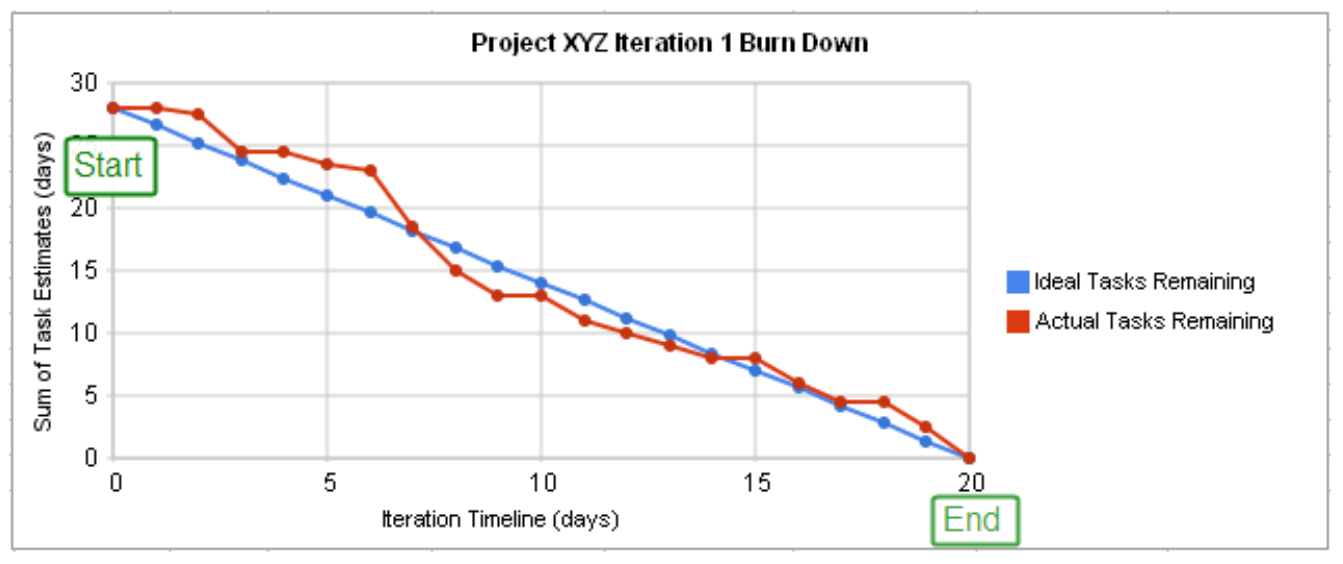
\includegraphics[width=\linewidth]{Immagini/burnDown}
	 \caption{Burndown Chart}
\end{figure}
Quello che faccio solitamente è tenere traccia dello scostamento rispetto alla pianificazione lineare.\\
Una approssimazione per calcolare il tempo nelle ascisse è usare i giorni uomo, ad esempio per un sprint di 2 settimane con sei programmatori abbiamo \texttt{6 programmatori \textbf{x} 5 giorni a settimana \textbf{x} 2 settimane \textbf{/} 3}. Il diviso 3 serve perchè i meeting ecc portano via circa un terzo della giornata.

\lessonDate{24 Ottobre 2019}
\section{Continuos Integration}
Nei primi anni dello sviluppo software si volevano seguire i modelli \textbf{Bottom Up} e \textbf{Top Down}. In realtà, sopratutto con l'object orientation, faccio tutto un po' alla cazzo, e non ho un chiaro modello di sviluppo.

\df{Continuos Integration}{Allineamento frequente (molte volte al giorno) dagli ambienti di lavoro degli sviluppatori verso l'ambiente condiviso (mainline)}

Questo modello porta alcune conseguenze:
\begin{itemize}
\item Non esiste una fase di integrazione definita, ma si integra via via per piccole parti. Questo però comporta che ogni volta che sviluppo una feature, essa debba essere integrabile.
\end{itemize}

\subsection{Capisaldi}
Martin Fowler nel 2006 formula alcuni principi:
\begin{itemize}
\item \textbf{Mantenere una singola repo}: ci deve essere tutto, dal codice alla documentazione. Devo avere anche una chiara visione di tutte le vecchie versioni del codice.
\item \textbf{Automatizzare la build}: già con make negli anni 70 era un problema. Ora con maven, gradle ecc siamo al top. In questo modo risparmio tempo e ho un processo più facile e affidabile.
\item \textbf{Build auto-testante}: Non scrivo parti di codice senza un minimo di test, quantomeno per non regredire
\item \textbf{Chiunque committa ogni giorno}: ad ogni commit di altre persone, integro i cambiamenti in modo tale da non avere problemi dopo. Siccome posso pushare solo dopo aver risolto i conflitti, l'integrazione avviene sulla mia macchina
\item \textbf{Ogni commit dovrebbe buildare sulla macchina di integrazione}: le build sono automatizzate. Se falliscono dei test, non consento il push
\item \textbf{Sistemo le build rotte subito}: se non riesco a sistemarla subito, faccio un revert e sistemo sulla mia macchina.
\item \textbf{Keep the build fast}: una build veloce permette di testare ad ogni commit
\item \textbf{Eseguire i test su un clone dell'ambiente di deployment}
\item \textbf{Rendere facile ottenere l'ultimo eseguibile}: il vecchio approccio era fornire solo le parti non generabili, quindi solo il sorgente. Potrebbe essere che con ambienti di sviluppo diversi il codice non compili. Quindi, bisogna fornire anche gli eseguibili.
\item \textbf{Tutti devono poter vedere cosa succede}: ovvero a che punto sono arrivato con lo sviluppo
\item \textbf{Automatic Deployment}
\end{itemize}

\subsection{Configuration Managment}
\noindent Dagli anni 70 comincia ad essere utilizzato nel mondo del software.
\df{Configuration Managment}{Pratiche che hanno l'obiettivo di rendere sistematico il processo di sviluppo, \textbf{tenendo traccia dei cambiamenti} in modo che il prodotto sia in ogni istante in uno stato (configurazione) ben definito.}
\noindent L'approccio iniziale era quello di versionare i singoli file, e non l'insieme. Inoltre, per la collaborazione venivano usati sistemi di write lock piuttosto scomodi.
\lessonDate{29 Ottobre 2019}\vspace{0.3cm}
\noindent \E meglio configurare l'insieme dei file e il loro stato, in modo tale da avere sempre una configurazione funzionale.\\
Quando lavoro sui file, calcolo le differenze in base alle linee di testo.\\
Dagli anni 2000, con l'avvento dell'open source e di internet, si sono resi necessari nuovi metodi di collaborazione \textbf{distribuiti} e \textbf{flessibili}, come git e mercurial. Questo è necessario a permettere una collaborazione da parte di molte persone e anche saltuaria.

\subsubsection{Artifact}
Ogni SCM deve affrontare alcune scelte:
\begin{itemize}
\item \textbf{Archiviazione degli artifact}: è molto costoso e occupa molto spazio, ma permette di avere esattamente il prodotto compilato. In alternativa, si può salvare meticolosamente la configurazione di ambiente per avere un processo di compilazione \textbf{replicabile}
\end{itemize}

\subsubsection{Sincronizzazione}
Il meccanismo base negli SCM è quello di \textbf{check-in} (commit) e \textbf{check-out}, che vanno a versionare un set di cambiamenti su uno o più file. Non vado quindi a versionare immediatamente ogni linea di codice. In teoria, non servirebbe un nodo centrale, perchè ogni peer possiede l'intera copia della codebase, che può essere sincronizzata con gli altri. In pratica, si usa un \textbf{repository centrale} per sincronizzare più velocemente e facilmente tutte le modifiche.

\subsubsection{Lavoro concorrente}
Si può gestire in due modi:
\begin{itemize}
\item \textbf{Lock:} ogni file ha un lock, e può essere modificato da una persona alla volta. Non il migliore approccio.
\item \textbf{Merge:} più persone possono modificare lo stesso file contemporaneamente, la prima persona che effettua il merge lo esegue, le altre risolvono i conflitti. \E possibile lavorare anche senza connessione, e poi posso sincronizzare in seguito.
\end{itemize}
\E chiaro che il \textbf{merge} è la tecnica superiore, anche se comunque a volte può essere difficoltoso. Posso avere varie situazioni:
\begin{itemize}
\item Lavoro parallelo su file diversi: non ho molti problemi, a meno che non faccio cazzate cambiando l'interfaccia.
\item Lavoro parallelo su hunk diversi: nessun problema, non creo conflitti.
\item Lavoro parallelo sullo stesso hunk: confitto :(, lo devo risolvere (ovviamente in locale) prima di pushare. Per capire chi abbia la versione modificata del file, vado a cercare un antenato comune fra la codebase A e la codebase B. Se A non presenta differenze e B si, allora vuol dire che è B che ha modificato il file.
\end{itemize}

\df{Hunk}{Insieme di righe adiacenti in file che hanno subito modifiche}

\subsubsection{Implementazione}
I vecchi sistemi di versioning salvavano ogni volta i \textbf{delta} dalla versione predente o successiva. Questo risparmia spazio, ma andare ad accedere a varie versioni è molto costoso. Git, invece, ogni volta che viene modificato un file lo salva nuovamente (compresso magari). Se invece un file non viene modificato, il file non viene aggiornato, basta aggiungere un nuovo puntatore.  Per capire se due file sono uguali, posso tranquillamente confrontare il loro hash, che mantengo sempre salvato come nome del file. Anche due file diversi ma in locazioni differenti sono salvati come puntatori allo stesso hash.

\section{Git}
Ci sono vari comandi base, non riportati qua, dei quali non verrà spiegato il funzionamento.
Il file fondamentale di \texttt{.git} è \texttt{HEAD} che mi dice qual'è la versione sulla quale sto lavorando.\\
I file memorizzati sono salvati con il loro hash dento \texttt{.git/objects}. Per velocizzare le perfomance, si usa il bucketing, ovvero si usano le prime due lettere del nome per raggruppare i file in cartelle. Ovviamente questi file sono compressi. I file più vecchi sono invece spostati nella cartella pack, dove non rompono le palle. Posso stampare e accedere a questi file con \texttt{git cat-file}.
\lessonDate{31 Ottobre}
Quando faccio add e poi modifico un file, la prima versione del file può rimanere memorizzata finchè git non decide di fare garbage collection.\\
Ogni file viene compresso con:
\begin{itemize}
\item \textbf{Header} comprendente tipo del file e dimensione
\item \textbf{Contenuto} del file
\end{itemize}
Git in realtà traccia i file in objects anche senza fare l'add. Se non vengono aggiunti, restano come dangling blobs, e vengono anche loro eliminati alla successiva garbage collection. I file che invece sono "indicizzati" sono visualizzabili da \texttt{git ls-files -s}.\\
Attenzione che le directory vuote non vengono tracciate! \E meglio pensare al nome dei file come al loro intero percorso, ex \texttt{dir1/dir2/file.txt}, e sono questi che vengono committati.\\
Ogni commit ha:
\begin{itemize}
\item Uno o più genitori (zero nel caso sono la radice)
\item Un \texttt{tree} con i file che ha linkato
\item Dei metadati, come committer ecc.
\end{itemize}
Quando committo, non vado a svuotare lo stage. Lo stage contiene tutto ciò che andrà nel prossimo commit (compresi i file già presenti).

\lessonDate{5 Novembre}
\vspace{1cm}
HEAD è il puntatore al punto di partenza alla working directory. Attraverso il comando \texttt{git tag}, posso taggare il branch corrente con un nome a mia scelta, in modo tale da poterlo trovare più velocemente. Posso usare il comando \texttt{git checkout nomeTag} per entrare all'interno del branch.\\
Posso riferirmi in vari modi a dei commit, come \texttt{tag}, \texttt{hash}, \texttt{HEAD} o \texttt{branch}. Posso anche riferirmi al padre (\texttt{cappuccio n}) o ad un antenato (\texttt{\textasciitilde n}).\\
Posso \textbf{riscrivere un commit} con \texttt{git commit --amend}, dimenticandomi così di mio padre.\\
\texttt{git reset [ref][--][files]} toglie le modifiche (fatte con \texttt{git add}) dallo stage, ma non le toglie dalla working directory. Se aggiungo \texttt{--files}, non vado a modificare la working dir, senza files sposto anche il branch puntato. Se uso \texttt{--hard}, tolgo i file anche dalla working dir. Con \texttt{--soft} non butto via ne la working dir, ne lo stage. Quindi, se puoi committo, sto praticamente facendo uno squash.

\lessonDate{7 Novembre}
\texttt{git revert} prende un commit precedente a quello attuale, e crea un nuovo commit che riporta al codice allo stato del suddetto commit.
\texttt{git bisect} mi permette di effettuare la bisezione per cercare la comparsa di una modifica all'interno del codice



\end{document}